\documentclass[11pt,a4paper]{report}
\usepackage[utf8]{inputenc}
\usepackage[portuguese]{babel}
\usepackage[T1]{fontenc}
\usepackage{amsmath}
\usepackage{amsfonts}
\usepackage{amssymb}
\usepackage{graphicx}
\usepackage{pgfplots}
\usepackage{float}
\pgfplotsset{compat=1.9}
\usepackage[left=2cm,right=2cm,top=2cm,bottom=2cm]{geometry}

\title{Processamento de Linguagens\\MIEI}

\author{
  Gonçalo Pereira\\
  \includegraphics[width=2cm]{a.jpeg}\\
  \texttt{A74413}
  \and
  António Silva\\
  \includegraphics[width=2cm]{b.jpeg}\\
  \texttt{A73827}
  \and
  André Diogo\\
  \includegraphics[width=2cm]{c.jpeg}\\
  \texttt{A75505}
}

\date{\today}

\begin{document}
\maketitle

\tableofcontents
\newpage


\chapter{Introdução}


\paragraph*{}Neste primeiro trabalho prático de Processamento de Linguagens, foi-nos pedida a realização de um filtro de texto para uma das quatro tarefas explicitadas, de modo a que fosse possível o reconhecimento de certos padrões de texto para uma correta transformação do ficheiro \texttt{.xml}. Como tal, escolhemos a realização de um filtro de texto para o exercício de \texttt{Transações de Via Verde}.

\paragraph*{}Após tal transformação do documento, ter-nos-ão sido incumbidas tarefas de \textit{parsing} do documento, maioritariamente de cálculo (número de entradas e total gasto), assim como as de escrita de listas de certos parâmetros. 

\paragraph*{}Como tal, e com este trabalho, demonstraremos como procedemos à realização de tais alíneas, demonstrando o que cada um dos \textit{scripts} de \texttt{AWK} faz, juntamente com a ilustração de exemplos.


\chapter{Processador de transações da Via Verde}


\section{Alínea A}


\paragraph*{}Nesta primeira alínea, foi-nos pedido o cálculo do número de entradas em cada dia do mês. Como tal, iniciámos pela filtragem de todos as \texttt{DATA_SAIDA}:

\begin{figure}[H]
\centering
\noindent\makebox[\textwidth]{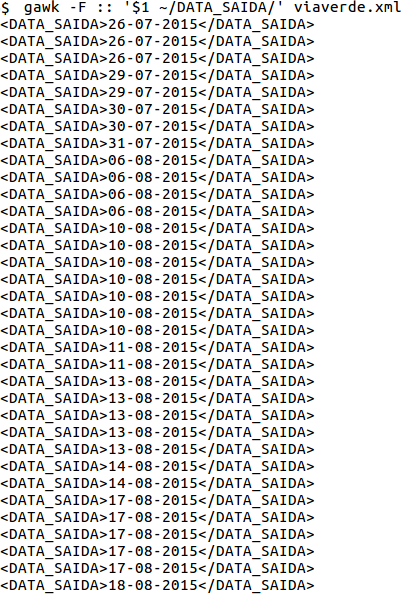
\includegraphics[width=\textwidth]{gawk_a1.png}}
\caption{Exemplo de dados obtidos pela execução do primeiro AWK, na bash.}
\end{figure}

\paragraph*{}De seguida, retirámos os duplicados e adicionámos as suas ocorrências, imprimindo-as com a sintaxe ilustrada pela seguinte imagem:

\begin{figure}[H]
\centering
\noindent\makebox[\textwidth]{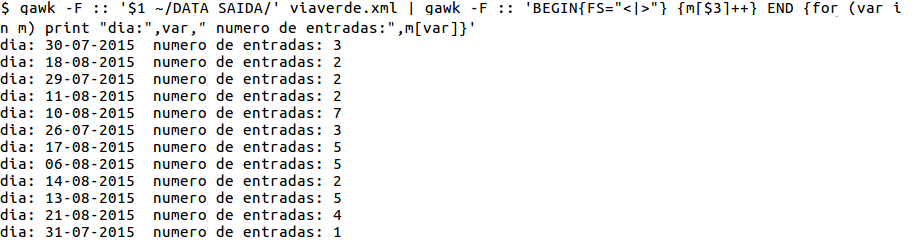
\includegraphics[width=\textwidth]{gawk_a2.png}}
\caption{Exemplo de dados obtidos pela execução do primeiro AWK, com o primeiro pipe, na bash.}
\end{figure}

\paragraph*{}Por fim, ordenámos o output obtido por ordem numérica, crescendo de mês a mês:

\begin{figure}[H]
\centering
\noindent\makebox[\textwidth]{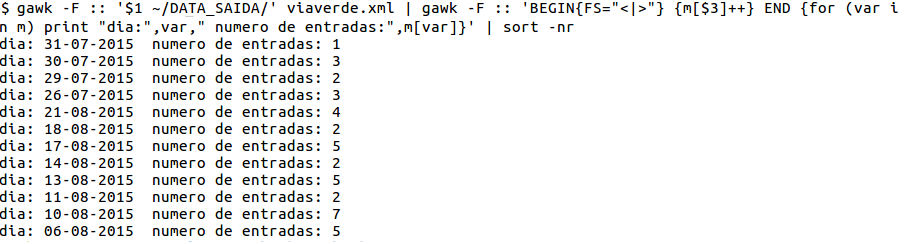
\includegraphics[width=\textwidth]{gawk_a3.png}}
\caption{Exemplo de dados obtidos pela execução do primeiro AWK, com o primeiro pipe e sort, na bash.}
\end{figure}

\paragraph*{}Após o trabalho efetuado na \texttt{bash} de texttt{UNIX}, convertemos a \textit{script} para um programa em \texttt{AWK}.

\begin{figure}[H]
\centering
\noindent\makebox[\textwidth]{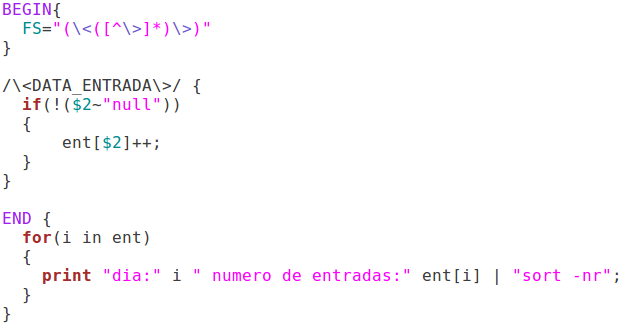
\includegraphics[width=\textwidth]{gawk_a4.png}}
\caption{Script final em AWK.}
\end{figure}


\section{Alínea B}


\paragraph*{}Na alínea b), seria objetivo a escrita de todos os locais de saída do extrato em específico. 	Primeiramente, filtrámos todos os parâmetros que estivessem incluídos na \textit{tag} de \texttt{<SAIDA>}, não excluíndo os duplicados.

\begin{figure}[H]
\centering
\noindent\makebox[\textwidth]{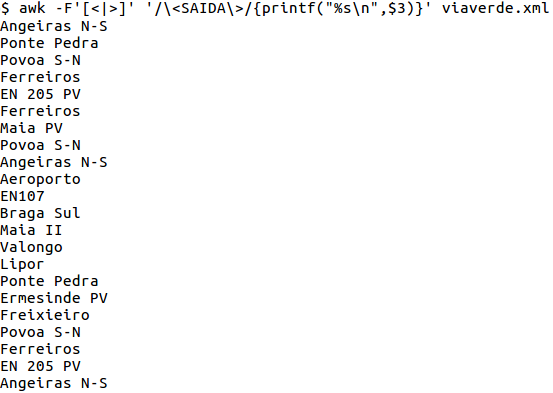
\includegraphics[width=\textwidth]{gawk_b1.png}}
\caption{Exemplo de dados obtidos pela execução do segundo AWK, na bash.}
\end{figure}

\paragraph*{}Seguidamente, filtrámos os duplicados de modo a que cada uma das saídas fosse impressa apenas uma vez:

\begin{figure}[H]
\centering
\noindent\makebox[\textwidth]{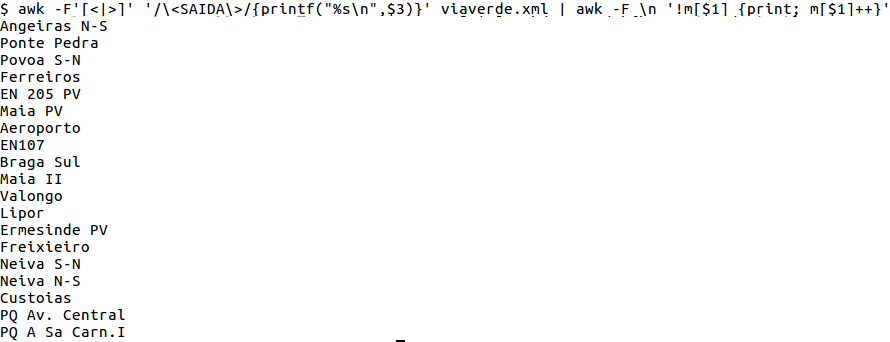
\includegraphics[width=\textwidth]{gawk_b2.png}}
\caption{Exemplo de dados obtidos pela execução do segundo AWK, com o primeiro pipe, na bash.}
\end{figure}

\paragraph*{}De igual modo, ordenámos as saídas por ordem alfabética, para que fosse de melhor compreensão:

\begin{figure}[H]
\centering
\noindent\makebox[\textwidth]{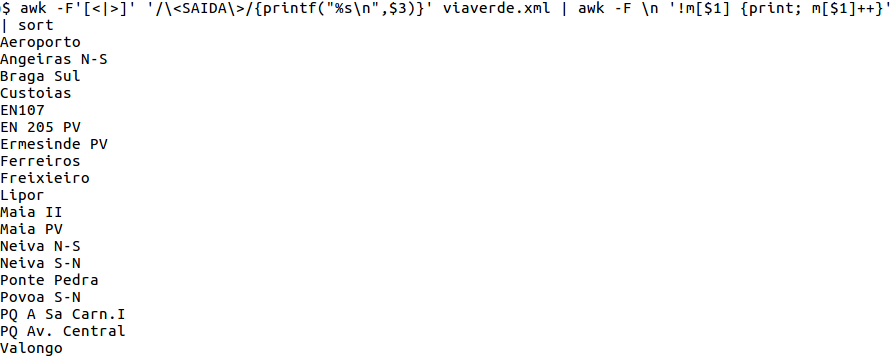
\includegraphics[width=\textwidth]{gawk_b3.png}}
\caption{Exemplo de dados obtidos pela execução do segundo AWK, com o primeiro pipe e sort, na bash.}
\end{figure}

\paragraph*{}Após o trabalho efetuado na \texttt{bash} de texttt{UNIX}, convertemos a \textit{script} para um programa em \texttt{AWK}.

\begin{figure}[H]
\centering
\noindent\makebox[\textwidth]{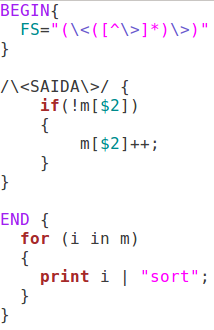
\includegraphics[width=\textwidth]{gawk_b4.png}}
\caption{Script final em AWK.}
\end{figure}


\section{Alínea C}


\paragraph*{}Nesta alínea ter-nos-á sido pedido o cálculo do total gasto em todo o mês. Em primeiro caso, começámos por filtrar todos os parâmetros que contivessem como \textit{tag}  \texttt{<IMPORTANCIA>}, com respetivos valores:

\begin{figure}[H]
\centering
\noindent\makebox[\textwidth]{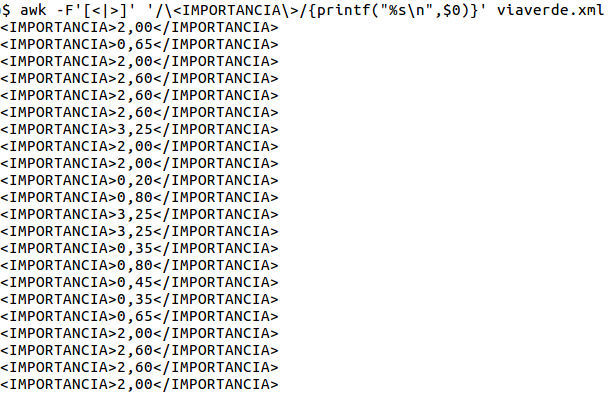
\includegraphics[width=\textwidth]{gawk_c1.png}}
\caption{Exemplo de dados obtidos pela execução do terceiro AWK, na bash.}
\end{figure}

\paragraph*{}Após esta filtragem, retirámos apenas os valores das importâncias para que pudessem ser somadas:

\begin{figure}[H]
\centering
\noindent\makebox[\textwidth]{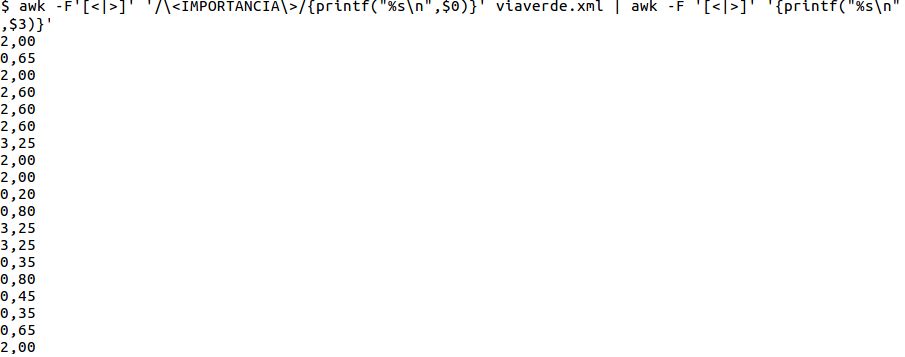
\includegraphics[width=\textwidth]{gawk_c2.png}}
\caption{Exemplo de dados obtidos pela execução do terceiro AWK, com o primeiro pipe, na bash.}
\end{figure}

\paragraph*{}Ultimamente, somámos todas as unidades e todos os cêntimos, sendo que estes últimos terão sido multiplicados por 100 (visto que a conversão é de 1 euro = 100 cêntimos):

\begin{figure}[H]
\centering
\noindent\makebox[\textwidth]{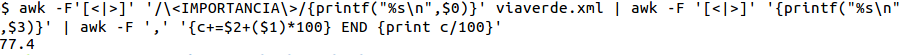
\includegraphics[width=\textwidth]{gawk_c3.png}}
\caption{Exemplo de dados obtidos pela execução do terceiro AWK, com o primeiro e segundo pipes, na bash.}
\end{figure}

\paragraph*{}Após o trabalho efetuado na \texttt{bash} de texttt{UNIX}, convertemos a \textit{script} para um programa em \texttt{AWK}.

\begin{figure}[H]
\centering
\noindent\makebox[\textwidth]{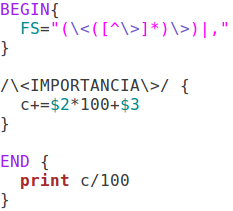
\includegraphics[width=\textwidth]{gawk_c4.png}}
\caption{Script final em AWK.}
\end{figure}


\section{Alínea D}


\paragraph*{}Na última alínea, a tarefa pedida terá sido semelhante à da alínea anterior, condicionando-se apenas de um modo: os totais gastos do mês serão apenas os gastos em parques. Assim, começámos por buscar todas as linhas de \textit{tag} com \texttt{IMPORTANCIA} e \texttt{TIPO}, alternadamente:

\begin{figure}[H]
\centering
\noindent\makebox[\textwidth]{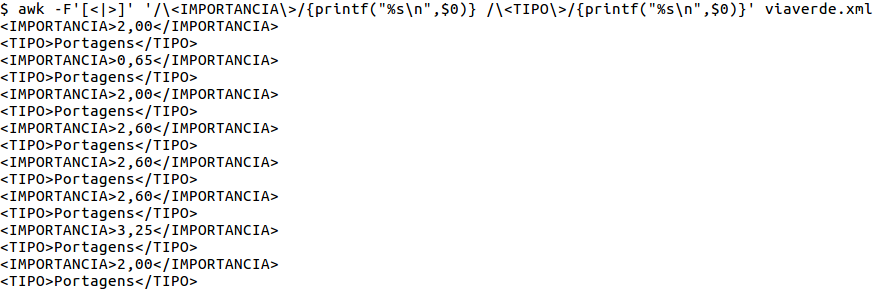
\includegraphics[width=\textwidth]{gawk_d1.png}}
\caption{Exemplo de dados obtidos pela execução do quarto AWK, na bash.}
\end{figure}

\paragraph*{}Depois, filtrámos as \textit{tags} e imprimimos cada duas linhas do passo anterior numa só, contendo a importância em euros e o tipo de ocorrência:

\begin{figure}[H]
\centering
\noindent\makebox[\textwidth]{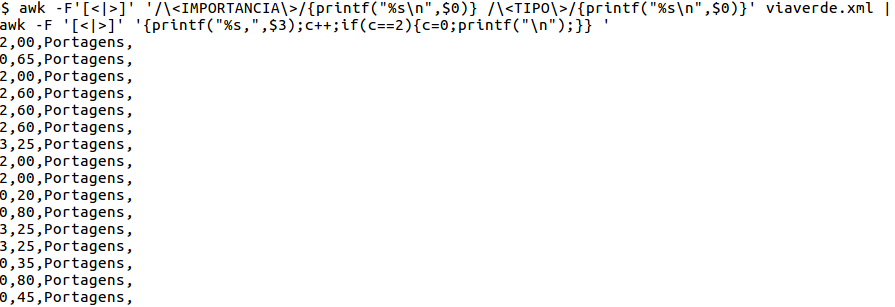
\includegraphics[width=\textwidth]{gawk_d2.png}}
\caption{Exemplo de dados obtidos pela execução do quarto AWK, com o primeiro pipe, na bash.}
\end{figure}

\paragraph*{}Finalizando, adicionámos um contador que somasse as importâncias que correspondessem ao tipo \texttt{Parque}. 

\begin{figure}[H]
\centering
\noindent\makebox[\textwidth]{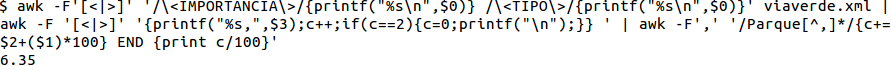
\includegraphics[width=\textwidth]{gawk_d3.png}}
\caption{Exemplo de dados obtidos pela execução do quarto AWK, com o primeiro e segundo pipes, na bash.}
\end{figure}

\paragraph*{}Após o trabalho efetuado na \texttt{bash} de texttt{UNIX}, convertemos a \textit{script} para um programa em \texttt{AWK}.

\begin{figure}[H]
\centering
\noindent\makebox[\textwidth]{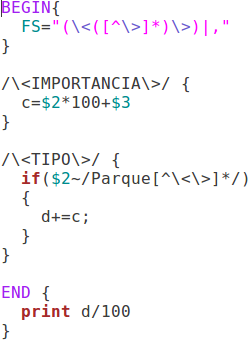
\includegraphics[width=\textwidth]{gawk_d4.png}}
\caption{Script final em AWK.}
\end{figure}


\chapter{Conclusão}

\end{document}
